% =============================================================================
% Crossbar Switch Chapter – Introduction / Concept
% Copy this into your Overleaf project.
% Required packages (add to your preamble if not already present):
%   \usepackage{tikz}
%   \usepackage{amsmath}
% =============================================================================

\section{Crossbar Switch}
\label{sec:crossbar}

\subsection{Concept and Operating Principle}
\label{subsec:crossbar_concept}

A crossbar switch is one of the most fundamental building blocks in network switch design.
Its purpose is to establish a configurable connection between any input port and any output port, 
allowing data to be routed from its source to its intended destination.
In its most general form, an $N \times N$ crossbar consists of a grid of $N^2$ crosspoints, 
where the $N$ horizontal input lines intersect with the $N$ vertical output lines.
Each crosspoint acts as a programmable switch that can be opened or closed: 
when a crosspoint at position $(i,\,j)$ is closed, input~$i$ is connected to output~$j$ 
and data flows through.
Figure~\ref{fig:classic_crossbar} illustrates this topology for a $4 \times 4$ configuration.

\begin{figure}[htbp]
    \centering
    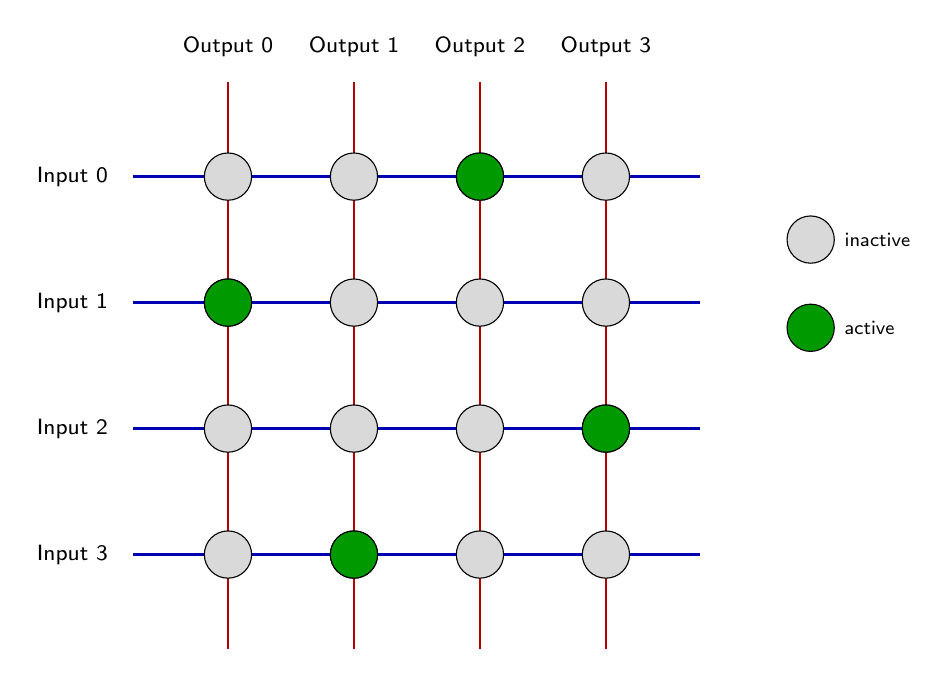
\begin{tikzpicture}[
        scale=1.0,
        crosspoint/.style={circle, draw, fill=black!15, minimum size=6mm, inner sep=0pt},
        crosspoint_active/.style={circle, draw, fill=green!60!black, minimum size=6mm, inner sep=0pt},
        port_label/.style={font=\footnotesize\sffamily},
    ]
    
    % Grid dimensions
    \def\N{4}
    \def\spacing{1.6}
    
    % Draw horizontal lines (inputs)
    \foreach \i in {0,...,3} {
        \draw[thick, blue!70!black] (-1.2, -\i*\spacing) -- (\N*\spacing - \spacing + 1.2, -\i*\spacing);
        \node[port_label, anchor=east] at (-1.4, -\i*\spacing) {Input \i};
    }
    
   \foreach \j in {0,...,3} {
        \draw[thick, red!70!black] (\j*\spacing, 1.2) -- (\j*\spacing, -3*\spacing - 1.2);
        \node[port_label, anchor=south] at (\j*\spacing, 1.4) {Output \j};
    }
    
    % Draw crosspoints (inactive)
    \foreach \i in {0,...,3} {
        \foreach \j in {0,...,3} {
            \node[crosspoint] at (\j*\spacing, -\i*\spacing) {};
        }
    }
    
    % Highlight active connections: 
    %   Input 0 -> Output 2,  Input 1 -> Output 0,  Input 2 -> Output 3,  Input 3 -> Output 1
    \node[crosspoint_active] at (2*\spacing, -0*\spacing) {};  % (0,2)
    \node[crosspoint_active] at (0*\spacing, -1*\spacing) {};  % (1,0)
    \node[crosspoint_active] at (3*\spacing, -2*\spacing) {};  % (2,3)
    \node[crosspoint_active] at (1*\spacing, -3*\spacing) {};  % (3,1)
    
    % Legend
    \node[crosspoint, label={[font=\scriptsize\sffamily]right: inactive}] at (\N*\spacing + 1.0, -0.5*\spacing) {};
    \node[crosspoint_active, label={[font=\scriptsize\sffamily]right: active}] at (\N*\spacing + 1.0, -1.2*\spacing) {};
    
    \end{tikzpicture}
    \caption{Classic $4 \times 4$ crossbar switch topology. Each intersection represents a 
    programmable crosspoint. Green (active) crosspoints indicate the currently established 
    connections: Input~0$\to$Output~2, Input~1$\to$Output~0, Input~2$\to$Output~3, 
    and Input~3$\to$Output~1.}
    \label{fig:classic_crossbar}
\end{figure}

A key property of the crossbar is its non-blocking nature: as long as no two inputs attempt to 
reach the same output simultaneously, all $N$ connections can be active in parallel without 
interference. However, when multiple input ports have data destined for the same output port, 
a conflict --- known as \emph{output contention} --- arises, and only one of the competing inputs 
can be served at any given time. Resolving these conflicts is the task of a 
\emph{scheduling algorithm}, which determines the crossbar configuration for each time slot.

In traditional input-queued (IQ) switch architectures, this scheduling problem is non-trivial. 
Algorithms such as iSLIP perform iterative matching between inputs and outputs over 
multiple rounds within a single clock cycle, which limits the achievable operating frequency 
--- particularly on FPGAs, where deep combinational logic paths directly reduce the maximum 
clock rate. The complexity grows further with the number of ports, as the scheduler must 
evaluate all possible input--output pairings.

The design presented in this work avoids this scheduling bottleneck entirely through the use 
of Virtual Output Queues (VOQs), which pre-sort incoming frames by their destination port 
\emph{before} they reach the crossbar. As a result, the crossbar itself can be implemented as a 
simple set of multiplexers rather than a dynamically scheduled switching matrix. This 
architectural simplification and its FPGA implementation are discussed in the following 
subsection.




% =============================================================================
% Crossbar Switch Chapter – Part 2: Simplified MUX-Based Architecture
% Copy this into your Overleaf project, directly after the introduction.
% Required packages (add to your preamble if not already present):
%   \usepackage{tikz}
%   \usetikzlibrary{positioning, arrows.meta, fit, calc, backgrounds}
% =============================================================================

\subsection{Simplified MUX-Based Crossbar Architecture}
\label{subsec:crossbar_simplified}

In a conventional input-queued switch, the crossbar must be able to establish arbitrary 
connections between any input and any output port in each time slot. This generality is what 
makes the scheduling problem difficult: a central scheduler must inspect all pending requests 
across all input ports, resolve output contention, and configure the entire $N \times N$ 
crossbar --- all within a single clock cycle. As the number of ports grows, this becomes a 
major bottleneck, especially on FPGAs where every additional level of combinational logic 
directly reduces the maximum achievable clock frequency.

The architecture presented in this work eliminates this problem by restructuring the data path 
\emph{before} the crossbar. As described in Section~\ref{sec:voq}, the design employs 
Virtual Output Queues that pre-sort incoming frames by destination port. In the $4 \times 4$ 
case, this results in $4 \times 4 = 16$ individual FIFOs, grouped by \emph{destination 
port} --- four FIFOs per output, one from each input.

Because all data arriving at a given output port's FIFO group is already guaranteed to be 
destined for that port, the crossbar no longer needs to perform arbitrary input-to-output 
routing. Each output port only needs to select \emph{which} of its four source FIFOs to 
read from at any given moment. This is a fundamentally simpler operation: instead of an 
$N \times N$ crossbar with $N^2$ configurable crosspoints, the switching fabric reduces to 
$N$ independent $N$-to-1 multiplexers, where each multiplexer serves exactly one output 
port.

The selection of which FIFO to read is handled by a dedicated round-robin arbiter per 
output port (see Section~\ref{sec:round_robin}), which outputs a 2-bit select signal 
(\texttt{rr\_sel}) that directly drives the corresponding multiplexer.
Figure~\ref{fig:voq_mux_arch} illustrates this architecture for a single output port. The 
same structure is replicated four times --- once for each output --- with each instance 
operating completely independently.

\begin{figure}[htbp]
    \centering
    \begin{tikzpicture}[
        >=Stealth,
        fifo/.style={
            draw, thick, minimum width=24mm, minimum height=8mm,
            fill=blue!8, font=\footnotesize\sffamily,
            rounded corners=1pt,
        },
        muxbox/.style={
            draw, thick, fill=orange!15, 
            minimum width=14mm, minimum height=55mm,
            font=\small\sffamily\bfseries,
            rounded corners=2pt,
        },
        rr/.style={
            draw, thick, fill=green!12, minimum width=26mm, minimum height=10mm,
            font=\footnotesize\sffamily, rounded corners=2pt,
        },
        data_arrow/.style={->, thick, blue!70!black},
        ctrl_arrow/.style={->, thick, red!70!black, dashed},
        grant_arrow/.style={->, thick, green!50!black, densely dotted},
        label_style/.style={font=\scriptsize\sffamily, text=black!70},
    ]

    % FIFOs — vertically spaced
    \node[fifo] (f0) at (0, 0)    {FIFO 0 \scriptsize(from In\,0)};
    \node[fifo] (f1) at (0, -1.4) {FIFO 1 \scriptsize(from In\,1)};
    \node[fifo] (f2) at (0, -2.8) {FIFO 2 \scriptsize(from In\,2)};
    \node[fifo] (f3) at (0, -4.3) {FIFO 3 \scriptsize(from In\,3)};

    % VOQ bundle box
    \begin{scope}[on background layer]
        \node[draw, dashed, thick, gray!60, fill=blue!3, rounded corners=4pt, 
              fit=(f0)(f3), inner xsep=5mm, inner ysep=3mm,
              label={[label_style, anchor=south]above:{%
                \normalsize\textsf{voq\_4to1 (Output Port $j$)}}}] (voq) {};
    \end{scope}

    % MUX — centred vertically between FIFOs
    \node[muxbox] (mux) at (5.5, -1.9) {4:1 MUX};

    % Output label
    \node[font=\sffamily\bfseries] (out) at (8.5, -1.4) {Output $j$};

    % Round-Robin Arbiter — below the VOQ box, horizontally centred 
    % between VOQ and MUX
    \node[rr] (rr) at (2.8, -6.2) {Round-Robin Arbiter};

    % ---- Data arrows: each FIFO -> MUX (all four go to the MUX, none through RR) ----
    \draw[data_arrow] (f0.east) -- (mux.west |- f0.east);
    \draw[data_arrow] (f1.east) -- (mux.west |- f1.east);
    \draw[data_arrow] (f2.east) -- (mux.west |- f2.east);
    % FIFO 3 routes around the RR box via a waypoint
    \draw[data_arrow] (f3.east) -- ++(1.2, 0) |- ($(mux.south west) + (0, 3mm)$);

    % ---- MUX -> Output ----
    \draw[data_arrow, very thick] (mux.east) -- (out.west)
        node[midway, above, label_style] {8-bit data};

    % ---- Control: RR --sel--> MUX ----
    \draw[ctrl_arrow, thick] (rr.east) -| (mux.south)
        node[pos=0.75, right=1mm, label_style, text=red!60!black] 
            {\texttt{rr\_sel} (2\,bit)};

    % ---- Control: FIFOs --frame_rdy--> RR ----
    \draw[ctrl_arrow, thick] ($(voq.south) + (-4mm, 0)$) -- ++(0, -0.5) 
        -- ($(rr.north) + (-4mm, 0)$)
        node[midway, left=1mm, label_style, text=red!60!black] 
            {\texttt{frame\_rdy} (4\,bit)};

    % ---- Grant: RR --rd_en--> FIFOs ----
    \draw[grant_arrow, thick] ($(rr.north) + (4mm, 0)$) -- ++(0, 0.5) 
        -- ($(voq.south) + (4mm, 0)$)
        node[midway, right=1mm, label_style, text=green!50!black] 
            {\texttt{rd\_en} / grant};

    \end{tikzpicture}
    \caption{Architecture of a single output port's datapath. The \texttt{voq\_4to1} module 
    groups four FIFOs (one per input port), all containing frames destined for the same output. 
    The round-robin arbiter selects which FIFO to read via a 2-bit select signal that drives 
    the 4:1 multiplexer. This structure is replicated independently for each of the four 
    output ports.}
    \label{fig:voq_mux_arch}
\end{figure}

This decomposition has several important consequences for the crossbar design. First, 
the output contention problem is resolved \emph{before} the crossbar stage: since each 
output port has its own dedicated FIFO group and arbiter, no two outputs ever compete 
for the same data path. Second, the crossbar itself becomes a purely combinational 
circuit with no internal state --- it is simply four independent multiplexers, each 
controlled by a 2-bit select line. Third, because every multiplexer operates 
independently and there is no shared scheduling logic, the design scales cleanly: 
adding more ports only adds more multiplexer instances without introducing 
cross-dependencies or longer critical paths.

Table~\ref{tab:crossbar_comparison} summarises the key architectural differences between 
a traditional scheduled crossbar and the VOQ-based multiplexer approach used in this design.

\begin{table}[htbp]
    \centering
    \caption{Comparison of a traditional scheduled crossbar versus the simplified 
    VOQ-based MUX architecture implemented in this design.}
    \label{tab:crossbar_comparison}
    \renewcommand{\arraystretch}{1.3}
    \begin{tabular}{l c c}
        \hline
        \textbf{Property} & \textbf{Traditional Crossbar} & \textbf{This Design} \\
        \hline
        Switching element     & $N^2$ crosspoints              & $N$ independent MUXes \\
        Scheduling algorithm  & iSLIP / maximal matching       & Simple round-robin per output \\
        Scheduler complexity  & $O(N^2)$ per iteration         & $O(N)$ total, no iterations \\
        Contention resolution & Centralised, iterative         & Distributed, per-output \\
        Critical path         & Scheduler + crossbar           & Single 4:1 MUX \\
        Internal state        & Configuration registers        & None (purely combinational) \\
        Data pre-sorting      & Not required                   & VOQs grouped by destination \\
        \hline
    \end{tabular}
\end{table}

In essence, the complexity that would normally reside in the crossbar's scheduling logic 
has been shifted upstream into the VOQ and round-robin stages (Sections~\ref{sec:voq} 
and~\ref{sec:round_robin}). What remains at the crossbar stage is the simplest possible 
switching operation: a multiplexer that forwards whichever input the arbiter has selected.